\chapter{Méthodes}
    \section{A*}


\subsection{Présentation rapide}

L'algorithme $A^*$ est un outil de recherche de plus court chemin dans un graphe. On peut l'utiliser pour résoudre des problèmes de type puzzle, en les ramenant à des problèmes de plus court chemin. Plus précisément dans le cas du Sudoku, on construit un graphe ayant pour racine la \textbf{grille initiale}, avec seulement les indications de départ.

Chaque sommet correspond ensuite à un état de la grille, parmi lesquels on avance en ajoutant un chiffre dans une case vide. On va donc de case en case jusqu'à ce que la grille soit complète ou que l'on ai trouvé une erreur, au quel cas on retourne en arrière et on retente une autre possibilité.

\bigskip

Sans revenir sur l'algorithme lui même, il est tout de même nécessaire de préciser certains points : $A^*$ utilise \textbf{deux listes}, une dites \textit{fermée} et l'autre \textit{ouverte}. \textit{La liste ouverte contient toute les cases vides et la liste fermée les cases contenant un chiffre.}

Pour déterminer quel chemin emprunter l'algorithme calcul un \textbf{coût} $F$ pour chaque sommet et cherche en cherche le minimum à chaque étape. \textit{Remarque : on calcule le coût de chaque case vide afin de déterminer laquelle est ``optimale'' pour continuer la recherche.} Le coût $F$ est déterminé comme la somme d'une fonction coût $G$ et d'une heuristique $H$.

\bigskip


La seule particularité de cette application de $A^*$ est que l'on doit, pour chaque case optimale choisie, tester toutes les possibilités de valeurs de possibles. Tant que l'on a pas trouvé de solution ou que l'on ai testé toute les grilles possibles, l'algorithme va :
\begin{itemize}
\item  actualiser les listes ouverte et fermée ainsi que les valeurs possibles des cases vides,
\item trouver la case ayant la plus petite valeur pour $F$,
\item créer des grilles à partir de la grille précédente \textit{(on assigne aussi celle-ci comme parent de la nouvelle grille)} et d'une des valeurs possibles pour la case ``optimale'',
\item vérifier la présence de doublon, si c'est le cas, il faut renvoyer une erreur, tester les autres possibilités et éventuellement remonter au niveau du parent pour essayer ses autres possibilités.
\item s'il n'y a pas de doublon, on recommence la recherche de case ``optimale'' dans la nouvelle grille \textit{(via récursivité)}

\end{itemize}



\subsection{Choix des fonctions coût}

On peut choisir différentes fonction coût pour le problème du Sudoku, ce choix va bien sur affecté le temps de calcul de l'algorithme.

\subsubsection*{La fonction G}

L'une des façons la plus simple de l'estimer est de prendre le nombre de cases vides dans la ligne, la colonne et le bloc contenant la case observée. En effet, moins il y a de case vide dans cette zone, plus il sera simple de déterminer une valeur.


\subsubsection*{L'heuristique H}

C'est principalement le choix de l'heuristique qui influe sur l'efficacité de l'algorithme, notre premier choix est une fonction qui renvoie le nombre de valeurs possibles pour la case testée \textit{(valeurs comprises entre $1$ et $9$)}.

Cette valeur est déterminée selon les règles du Sudoku \textit{(une seule apparition par ligne, colonne ou bloc)} et les cases contenues dans la liste fermée \textit{(les cases remplies de la grille)}.

\textit{Remarque : dans le cas où il n'y a aucune possibilité, c'est que l'on a trouvé une erreur, on renverra alors la valeur $9$ ainsi qu'un message d'erreur.}




\subsection{Implémentation}

\subsubsection{Diagramme de classe}

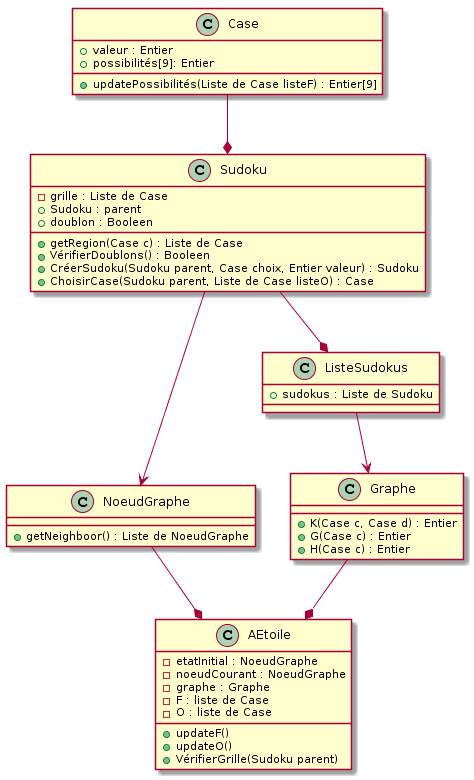
\includegraphics[scale = 0.5]{images/AstarDiagrammeClasse.png}

\bigskip


\begin{description}
\item[Case :] 
C'est un emplacement pouvant recevoir une \textit{valeur} comprise entre $1$ et $9$. Chaque Case possède un tableau de $9$ entiers \textit{possibilités[]}, initialisé à $\{1,2,3,4,5,6,7,8,9\}$.

La fonction \textit{updatePossibilités()} met à jour les valeurs possibles de la Case, en fonction des Cases contenues dans la liste fermée. Si une valeur est impossible, on la remplace par $0$ dans \textit{possibilités[]}.


\item[Sudoku :] Il s'agit tout d'abord d'une \textit{grille}, une liste de 81 Cases, ainsi qu'un booléen \textit{doublon}. On utilise aussi une référence au Sudoku \textit{parent}, celui qui à permit d'obtenir ce Sudoku.

La fonction \textit{getRégrion(Case c)} renvoie la liste des autres Cases contenues dans la même région que la Case c \textit{(dans la ligne, la colonne et le bloc)}.

Comme son nom l'indique, \textit{VérifierDoublon()} va tester la présence de doublon dans une ligne, une colonne ou un bloc de la grille.

\textit{CréerSudoku(Sudoku parent, Case choix, Entier valeur)} construit un nouveau Sudoku à partir du Sudoku \textit{parent}, en lui ajoutant le chiffre \textit{valeur} dans la Case vide \textit{choix}.

Enfin, \textit{ChoisirCase(Sudoku parent, Liste de Case listeO)} détermine quelle Case de \textit{listeO} est ``optimale'' pour le prochain déplacement depuis \textit{parent}, c'est ici que l'on va chercher le minimum de $F=G+H$.

\textit{La classe Sudoku hérite de la classe NoeudGraphe, contenant un fonction qui renvoie les NoeudGraphes voisins d'un NoeudGraphe.}


\item[ListeSudokus : ] On maintient simplement une liste de tout les Sudokus construis.

\textit{ListeSudokus hérite de la classe Graphe, qui contient les méthodes permettant de calculer $G$ et $H$}

\item[AEtoile :] Possède un \textit{etatInitial}, le NoeudGraphe qui correspond à la grille de départ, un Graphe et un NoeudGraphe \textit{noeudCourant}. C'est dans cette classe que sont définit les listes de Cases \textit{listeFermée} et \textit{listeeOuverte}, ainsi que les méthodes pour les mettre à jour.

La fonction \textit{VérifierGrille(Sudoku parent)} est la fonction récursive principale de l'algorithme, celle qui va appeler \textit{ChoisirCase()}, \textit{CréerSudoku()} et \textit{VérifierDoublon()}.



\end{description}


\subsubsection{Diagramme de séquences}

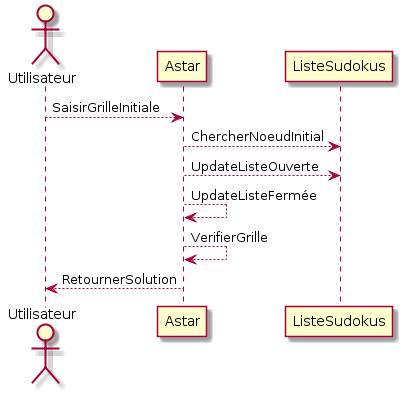
\includegraphics[scale=0.5]{images/AstarDiagrammeSequences.png}



    \section{Algorithme génétique}
        \subsection{Généralité}
            Les algorithmes génétiques sont des algorithme basés sur là représentation de l'évolution dans la génétique.\\
            En premier lieu, l'algorithme va créer un ensemble d'individu, au propriétés aléatoires.
            Par la suite, l'algorithme va dérouler 3 phases bien distinctes, jusqu'à arriver à un individu qui répondra complètement au problème: 
            \begin{itemize}
                \item \textbf{Sélection}: parmi tous les individus présents, seuls les plus pertinents (Ceux dont la fonction de \textbf{fitness} sera la plus grande) seront gardés.
                \item \textbf{Croisement}: une fois les individus choisis, il faut les utiliser Pour recréer un nouvel ensemble d'individu plus aptes, \textbf{réutilisant les gènes des parents} présents.\\
                    La manière dont le croisement est fait dépend du problème.
                \item \textbf{Mutation}: Une fois notre nouvelle espèce créée, chaque individu se verra ajouter \textbf{une part d'aléatoire} dans son génome.
            \end{itemize}
            Voyons en détails ces trois étapes.
        \subsection{Sélection}
            Comme dit précédemment, une sélection se fait sur les individus présents.\\
            Au même titre que pour $A^*$, il nous faut définir une échelle qui nous permettra de comparer les individus entre eux pour déterminer quels sont ceux les plus à même d'apporter des bribes de réponse à notre problème.\\
            Nous allons donc définir pour chaque problème une \textbf{fonction fitness} qui prendra le génome de l'individu, et qui en donnera un score, totalement indépendant d'autre facteur.\\
            Dans notre cas, nous aborderons le sujet plus tard, mais cela pourrai par exemple être le nombre de conflit présents sur une grille donnée (Auquel cas il faudrait non plus maximiser cette fonction, mais la minimiser)
        \subsection{Croisement}
            Les croisement a pour intérêt de créer une nouvelle population, qui ne sera pas aléatoire (contrairement à la première), mais qui utilisera les attributs de ces meilleurs prédécesseurs.\\
            la manière la plus simple de voir une telle chose, est en représentant chacun des génomes par un tableau d'entier.\\
            Avec deux tels parents, on peut facilement créer un mélange entre les deux (En prenant par exemple la moitié de chaque tableaux, ce qui nous donnera 2 enfants).\\
            Le piège est malgré tout de croiser intelligemment.\\
            En effet, si pour notre problème de Sudoku, nous prenions 1 case sur 2 pour faire le croisement, cela n'assurera en rien d'avoir des enfants dont le score risque de monter.
        \subsection{Mutation}
            Le dernier stade, et le plus ``crucial'' reste la mutation.\\
            En effet, même après avoir croisé l'ensemble des gènes des parents, ils se peut qu'il manquerait un gène pour résoudre le problème.\\
            C'est la raison pour laquelle chacun de nos enfants se verra modifié de manière aléatoire un ou plusieurs de ces gènes.
    \section{Résolution humaine}



        L'idée est d'implémenter un algorithme qui résout le Sudoku en utilisant les mêmes méthodes de résolution qu'un humain. L'algorithme définit simplement un ensemble de règles qui permette la résolution progressive du Sudoku. Revenons sur ces règles plus en détails :

        \begin{description}
       \item[Le singleton :] c'est le cas le plus simple, ou il ne reste qu'une seule case vide dans une ligne, une colonne ou un bloc, on peut alors directement déterminer la valeur manquante.

        \item[L'élimination directe :] \textit{Quelles cases dans cette ligne, colonne ou bloc, peut contenir telle valeur ?} On peut déterminer la position d'une valeur dans une région par élimination, c'est bien sur plus facile si la valeur est déjà fréquente dans la grille.

        \item[Les possibilités uniques :] c'est la recherche de cases n'ayant qu'une seule possibilité de valeur, car toutes les autres sont déjà présentes dans sa région.

        \item[L'élimination indirecte :] quand on utilise les propriétés d'une ligne ou colonne et celle d'un bloc pour déterminer la position d'une valeur dans ce bloc. Si à l'intérieur d'un bloc on peut isoler une valeur dans une ligne ou colonne, on peut alors savoir qu'elle n'apparaitra pas dans cette même ligne ou colonne au sein d'un autre bloc.

       \item[La reconnaissance de motifs :] il existe des techniques plus avancées qui se basent qur la reconnaissance de motifs simples dans une grille qui permettent d'identifier la position d'une valeur.


        \end{description}

\textit{Remarque : on peut utiliser ces règles pour améliorer la recherche de case optimale dans $A^*$ par exemple.}






	\section{Eco-résolution}
    \subsection{Principe de résolution}
        L'éco-résolution est une méthode de résolution de problème qui prend le contre-pied des techniques classiques. Plutôt que de résonner que manière globale et définir des méthodes de résolution, l'éco-résolution préfère considérer le problème comme des agents en interactions devant satisfaire un but. \\ \\
        Il faut donc pour pouvoir appliquer l'éco-résolution définir un ensemble d'agents dont le but est de tendre vers un état stable (solution du problème). Chaque agent répond à deux principes importants: autonomie et localité. C'est à dire que chaque agent agit de manière locale mais aussi en fonction des interactions qu'il a avec les différents agents avec lesquels il est en relation.
        Les particularités de l'éco-résolution sont les suivantes:
        \begin{itemize}
        \item Pas d'exploration globale de l'ensemble des états. Seuls les états des différents agents sont pris en compte. 
        \item Résiste très bien au bruit: une perturbation ne modifie que peu le mécanisme de résolution, en effet c'est une donnée normale dans le principe de résolution.
        \item De ce fait permet de résoudre des problèmes de grand taille. 
        \end{itemize}
    
	\subsection{Les éco-agents}
        Les agents disposent d'un ensemble de comportements élémentaires qui les pousse à rechercher un état de satisfaction. Quand un agent est en état de recherche de satisfaction, ils peuvent être gênés par d'autres agents. Dans ce cas, ils agressent les gêneurs, ces derniers devant fuir.  Dans leur fuite, ils peuvent être amenés à agresser d'autres agents les empêchant de fuir, cette opération se poursuivant jusqu'à ce que tous les gêneurs bougent. \\
        \\
        Chaque éco-agent est défini par les éléments suivants:
        \begin{itemize}
        \item Un but, relation particulière avec d'autres agents : relation de satisfaction 
        \item Un état interne:  Un éco-agent peut-être dans un des quatre états-suivants : satisfaction, recherche de satisfaction, recherche de fuite ou fuite. 
        \item Fonction de perception de gêneurs, ensemble des gêneurs qui empêche l'agent d'être satisfait ou de fuir. 
        \item Actions élémentaires, dépendant de l'application, qui définissent la satisfaction et la fuite. 
        \item Les dépendances sont les agents dont l'agent courant est le but. Ces dépendances ne pourront être satisfaites que si l'agent courant est satisfait. Ces dépendances dépendent donc des relations de satisfaction.
        \end{itemize}
        
        \begin{itemize}
        \item  Volonté d'être satisfait : les eco-agents cherchent à se trouver dans un état de satisfaction. S'ils ne sont pas dans un état de satisfaction, ils agressent les gêneurs. \\
        \begin{verbatim}
        Procédure seSatisfaire(x) 
        si le but de x nest pas satisfait alors 
        pour tous les agents y qui gênent x 
        agresser(y,but(x))
        des qu'il n'y a plus de gêneurs alors 
        faire satisfaction(x)
        \end{verbatim}
        La fonction faireSatisfaction dépend du domaine d'application. Execute l'opération donc le résultat aura pour conséquence que l'agent vérifie sa condition de satisfaction. La fonction agression consiste à ce que l'agent y fuis l'agent x en s'éloignant de son objectif.  
        \item L'obligation de fuir. Lorsqu'un eco-agent est attaqué il est obligé de fuir. Il doit choisir une satisfaction qui satisfasse la contrainte passée en argument de la fonction fuir. \\
       \begin{verbatim}
        Procedure fuir(y,c)    notre agent(x) fuis y avec la contrainte c
        si x etait satisfait, x devient insatisfait 
        soit p=trouverPlacePourFuir(x,y,c) 
        si p = Nil alors "pas de solution"
        sinon \\
            pour tous les agents z qui gênent x dans sa fuite vers p 
            fuir (z,x,p) 
            des qu il n'y a plus de gêneurs pour fuir
            alors faireFuite(x,p) 
        \end{verbatim}    
        Les fonction trouverPlacePourFuir et faireFuite dépendent de l'application. La première cherche une place dans l'environnement où l'agent peut fuir et la seconde réalise effectivement l'action de fuite.     
        \end{itemize}
    
    
    
        \subsection{L'eco-resolution vu comme un automate}
        Il est possible de voir la résolution comme étant un automate à états finis comme suit : \\
\begin{center}
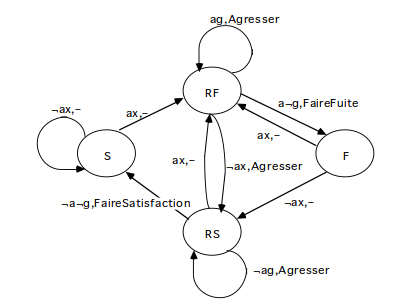
\includegraphics[scale=0.7]{images/AutomateEcoResolution.png}
\end{center}
Les quatres états sont les suivants : satisfaction (S), fuite (F), recherche de satisfaction (RS) et recherche de fuite (RF). a et g représentent respectivement une agression et un gêne, -a représentant l'absence d'agression. Le dernier paramètre représente l'action effectuée. \\
\\
Si notre agent est en état de \textbf{recherche de satisfaction}, il y a trois possibilités. \\
\begin{itemize}
\item Il n'est pas agressé ni gêné pour atteindre son but, il effectue donc FaireSatisfaction pour se trouver en état de \textbf{Satisfaction}.
\item Il n'est pas agressé mais il est gêné par un autre agent pour atteindre son but, il agresse donc le gêneur et reste en état de \textbf{Recherche de satisfaction}.
\item Il est agressé par un autre gêneur, il passe donc en \textbf{Recherche de fuite}
\end{itemize} ~\\
~\\
Deuxième possibilité, notre agent est en \textbf{Recherche de Fuite}, nous avons trois possibilités également. \\
\begin{itemize}
\item Il n'est pas gêné pour fuir, il exécute donc l'action FaireFuite et se retrouve dans l'état de \textbf{Fuite}
\item Il est gêné pour fuir, il va donc agressé les différents eco-agents qui le gêne. Tant qu'il sera gêné et agressé il restera dans l'état de \textbf{Recherche de Fuite}
\item Il se retrouve à ne plus être agressé mais il n'a pas fuit, il passe donc en état de \textbf{Recherche de Satisfaction} 
\end{itemize}~\\
~\\
Troisième possibilité, notre agent est en état de \textbf{satisfaction}, il y a donc deux possibilités :\\
\begin{itemize}
\item Il n'est pas agressé il reste donc dans son état de \textbf{satisfaction} car il ne sera pas gêné.
\item Il est agressé et passe donc en état de \textbf{Recherche de fuite}. 
\end{itemize}~\\
~\\
Et enfin, il est en état de \textbf{Fuite}, on a les possibilités suivantes :\\
\begin{itemize}
\item Il est agressé et se retrouve donc en état de \textbf{Recherche de Fuite}
\item Il n'est pas agressé et est donc en état de \textbf{Recherche de Satisfaction}
\end{itemize}
